\chapter{Characterizing Equivalent Inputs}

When considering an LELM device, it's convenient to break the device into two components: the linear evolution section, which is comprised of the $L$ and $R$ channels as well as the transformations $U_L$ and $U_R$, and the local measurement section, which is comprised of the $2d$ detection modes. In this chapter, we are completely concerned with inputs into our LELM device and what can be done on them by local operations. We focus on the question of which subsets of a Bell basis can be transformed into one another using only local operations (if so, we call these sets \textit{equivalent}).

This question of determining equivalence classes of input sets is interesting in its own right, but is also useful for proving indistinguishably results. Once we prove that some subset of Bell states cannot be distinguished by and LELM device, we've shown that no equivalent subset can be distinguished by an LELM device. Generally, we hope to find that the equivalence classes are as large as possible since then results about particular sets of Bell states carry the most weight.

\begin{figure}
\centering
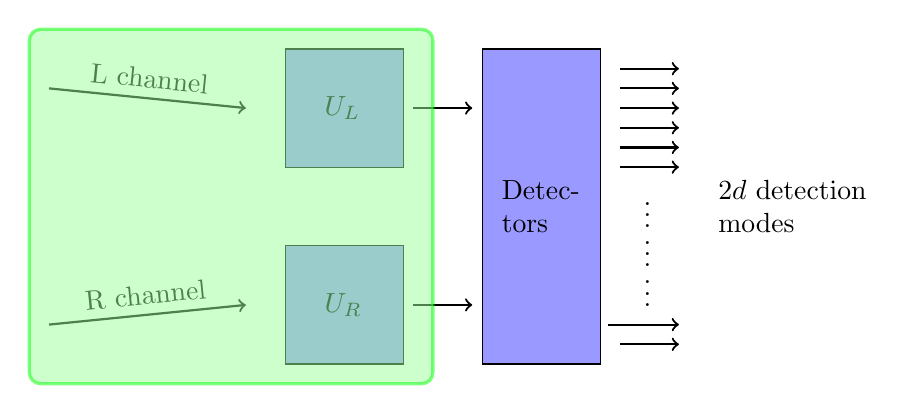
\begin{tikzpicture}
\filldraw[fill=blue!40!white, draw=black] (2.5,0) rectangle (4,4);
\filldraw[fill=blue!40!white, draw=black] (0,0) rectangle (1.5,1.5);
\filldraw[fill=blue!40!white, draw=black] (0,2.5) rectangle (1.5,4);
\draw[thick,->] (-3,3.5) -- (-0.5,3.25) node[midway, above, sloped] {L channel};
\draw[thick,->] (-3,0.5) -- (-0.5,0.75) node[midway, above, sloped] {R channel};
\node[text width=3cm] at (2, 0.75) {$U_{\text{R}}$};
\node[text width=3cm] at (2, 3.25) {$U_{\text{L}}$};
\node[text width=1cm] at (3.25, 2) {Detec- tors};


\draw[thick,->] (1.625,3.25) -- (2.375,3.25);
\draw[thick,->] (1.625,0.75) -- (2.375,0.75);

\draw[thick,->] (4.25,3.75) -- (5,3.75) node[midway, above] {};
\draw[thick,->] (4.25,3.5) -- (5,3.5) node[midway, above] {};
\draw[thick,->] (4.25,3.25) -- (5,3.25) node[midway, above] {};
\draw[thick,->] (4.25,3.0) -- (5,3.0) node[midway, above] {};
\draw[thick,->] (4.25,2.75) -- (5,2.75) node[midway, above] {};
\draw[thick,->] (4.25,2.5) -- (5,2.5) node[midway, above] {};
\node (A) at (4.6,2) {$\vdots$};
\node (A) at (4.6,1.5) {$\vdots$};
\node (A) at (4.6,1) {$\vdots$};
\draw[thick,->] (4.1,0.5) -- (5,0.5) node[midway, above] {};
\draw[thick,->] (4.25,0.25) -- (5,0.25) node[midway, above] {};
\node[text width=2cm] (A) at (6.5,2) {$2d$ detection modes};

\filldraw[fill=green!40!white, opacity=0.5, draw=green, very thick, rounded corners] (-3.25,-0.25) rectangle (1.875,4.25);

\end{tikzpicture}
\label{fig:inputs}
\caption{An LELM device, with the focus of this chapter highlighted in green.}
\end{figure}

\section{A Group of Transformations}

One approach to answering the question "What subsets of the Bell bases can be transformed into each other by local operations?" is to look at transformations of the form $U_L \otimes U_R$ that permute the Bell basis. In his senior thesis, Nathaniel Leslie presents a set of four transformations for the $d = 3$ case that permute the Bell basis. Each transformation has a simple corresponding description in terms of tic-tac-toe diagrams. The four rotations that Nathaniel looked at were:

\begin{enumerate}
  \item[$\hat{i}_p$:] Cycle all the columns right.
  \item[$\hat{i}_c$:] Cycle all the rows down.
  \item[$\hat{s}_p$:] Shift the rows in a staggered manner. Leave the first ($c = 0$) row unchanged. Move the second ($c = 1)$ row one to the right. Move the third ($c = 2$) row two to the right. [Note: moving a row two the right is the same as moving it one to the left.]
  \item[$\hat{s}_c$:] Move the columns in a staggered manner. Leave the first ($p = 0$) column unchanged. Move the second ($p = 1$) column one down. Move the third ($p = 2$) column two down.
\end{enumerate}

We've chosen to name these four translations $\hat{i}_p$, $\hat{i}_c$, $\hat{s}_p$, $\hat{s}_c$ for increment phase, increment correlation class, stagger phase, stagger correlation class. The way we have defined these transformations is in terms of our diagram, so we need to describe them in terms of separate operations on left and right channel particles, which we will do shortly. But first, it's useful to see how the group generated by these simple transformations acts on subsets of the Bell basis. Let $G_d = \langle i_p, i_c, s_p, s_c \rangle$ and let $S = \{\ket{\Psi_0^0}, \ket{\Psi_0^1}, \ket{\Psi_0^2}, \ket{\Psi_1^2}\}$, the subset from Figure \ref{fig:actions}, which also depicts the same set $S$ after the operations $\hat{i}_p,\; \hat{i}_c,\; \hat{s}_p,$ and $\hat{s}_c$.

\begin{figure}
\centering
\begin{tikzpicture}

\node[text width=3cm] at (3, 3.5) {$\hat{i}_p$};
\draw[step=1cm,thick] (0,0) grid (3,3);
\draw (0.5,2.5) node[cross=0.25cm,green, thick] {};
\draw (1.5,2.5) node[cross=0.25cm,red, thick] {};
\draw (2.5,2.5) node[cross=0.25cm,blue, thick] {};
\draw (0.5,1.5) node[cross=0.25cm,orange, thick] {};

\node[text width=3cm] at (7, 3.5) {$\hat{i}_c$};
\draw[step=1cm,thick] (4,0) grid (7,3);
\draw (4.5,1.5) node[cross=0.25cm,red, thick] {};
\draw (5.5,1.5) node[cross=0.25cm,blue, thick] {};
\draw (6.5,1.5) node[cross=0.25cm,green, thick] {};
\draw (6.5,0.5) node[cross=0.25cm,orange, thick] {};

\node[text width=3cm] at (11, 3.5) {$\hat{s}_p$};
\draw[step=1cm,thick] (8,0) grid (11,3);
\draw (8.5,2.5) node[cross=0.25cm,red, thick] {};
\draw (9.5,2.5) node[cross=0.25cm,green, thick] {};
\draw (10.5,2.5) node[cross=0.25cm,blue, thick] {};
\draw (8.5,1.5) node[cross=0.25cm,orange, thick] {};

\node[text width=3cm] at (15, 3.5) {$\hat{s}_c$};
\draw[step=1cm,thick] (12,0) grid (15,3);
\draw (12.5,2.5) node[cross=0.25cm,red, thick] {};
\draw (13.5,1.5) node[cross=0.25cm,blue, thick] {};
\draw (14.5,2.5) node[cross=0.25cm,orange, thick] {};
\draw (14.5,0.5) node[cross=0.25cm,green, thick] {};

\draw[step=1cm,thick] (6,4) grid (9,7);
\draw (6.5,6.5) node[cross=0.25cm,red, thick] {};
\draw (7.5,6.5) node[cross=0.25cm,blue, thick] {};
\draw (8.5,6.5) node[cross=0.25cm,green, thick] {};
\draw (8.5,5.5) node[cross=0.25cm,orange, thick] {};
\end{tikzpicture}
\caption{Some basic actions on $S = \{\ket{\Psi_0^0}, \ket{\Psi_0^1}, \ket{\Psi_0^2}, \ket{\Psi_1^2}\}$}
\label{fig:actions}
\end{figure}

Another way we can describe these transformations is by what they send a generic state to:

\begin{enumerate}
  \item[$\hat{i}_p$:] $\ket{\Psi_c^p} \rightarrow \ket{\Psi_c^{p+1}}$
  \item[$\hat{i}_c$:] $\ket{\Psi_c^p} \rightarrow \ket{\Psi_{c+1}^p}$
  \item[$\hat{s}_p$:] $\ket{\Psi_c^p} \rightarrow \ket{\Psi_c^{p+c}}$
  \item[$\hat{s}_c$:] $\ket{\Psi_c^p} \rightarrow \ket{\Psi_{c+p}^p}$
\end{enumerate}

%TODO: Make explicit transition from d = 3 to general d

\subsection{Defining the Transformations}
Now it's time for us to define the transformations $\hat{i}_p, \hat{i}_c, \hat{s}_p$, and $\hat{s}_c$ in terms of operations on single-particles. Here, we'll switch to a more condensed notation for denoting which channel a particle came from, using a subscript. As usual, arithmetic is done $\text{mod } d$. 
\begin{enumerate}
  \item[$\hat{i}_p$:] To do this transformation, we cycle the phase in the left channel:
  \[
  \hat{i}_c \ket{k}_L \rightarrow \omega^k \ket{k}_L \quad \text{and} \quad \hat{i}_c \ket{k}_R \rightarrow \ket{k}_R
  \]
  where $\omega = e^{i 2 \pi / d}$. This increments the phase.
  \item[$\hat{i}_c$:] To do this transformation, we cycle the variable in the right channel:
  \[
  \hat{i}_p \ket{k}_L \rightarrow \ket{k}_L \quad \text{and} \quad \hat{i}_p \ket{k}_R \rightarrow \ket{k + 1}_R.
  \]
  This increments the correlation class.
  \item[$\hat{s}_p$:] This transformation is trickier, so we'll show how to derive it. Instead of simply guessing the solution like for the incrementing transformations, we'll begin by describing symbolically a semi-generic transformation on the left channel particle looks like.\footnote{By semi-generic, we mean that we will restrict ourselves to looking at the subset transformations where the correlation class is fixed but the resulting phases are completely generic.} The free variables in this our description (i.e. $x_0, x_1, \ldots, x_{d-1}$) represent information about how the phase of each left-particle ket changes. They're defined as such:
\begin{equation}
\begin{split}
    \hat{s}_p \ket{0}_L & \rightarrow \omega^x_0 \ket{0}_L \\
    \hat{s}_p \ket{1}_L & \rightarrow \omega^x_1 \ket{1}_L \\
    & \; \; \vdots \\
    \hat{s}_p \ket{d-1}_L & \rightarrow \omega^x_{d-1}\ket{d-1}_L
\end{split}
\end{equation}

Next, we'll derive from our desired behavior of $\hat{s}_p$ what the values we need for our $x_i$'s. Since $\hat{s}_p \ket{\Psi_0^p} = \ket{\Psi_0^{p+0}} = \ket{\Psi_0^p}$, then we must have that $\hat{s}_p \ket{d-1}_R \rightarrow \omega^{-x_{d-1}}\ket{d-1}_R$. This guarantees that $\hat{s}_p \ket{(d-1)(d-1)} \rightarrow \omega^{-x_{d-1}}\omega^{x_{d-1}} \ket{(d-1)(d-1)} = \ket{(d-1)(d-1)}$.

  Now, setting $c=1$ gives us a system of equations. We want $\hat{s}_p$ to increment by $1$, up to an overall phase of $\frac{dy}{2 \pi}$, meaning:
\begin{equation}
  \begin{split}
        \hat{s}_p \ket{\Psi_1^p} &= \hat{s}_p  \pn{ \frac{1}{\sqrt{d}}\pn{\ket{0}_L\ket{1}_R + \omega^{p} \ket{1}_L\ket{2}_R + \omega^{2 p} \ket{2}_L\ket{3}_R + \cdots + \omega^{(d-1)p} \ket{d-1}_L\ket{0}_R} } \\
                             &= \frac{\omega^{y}}{\sqrt{d}}\pn{\ket{0}_L\ket{1}_R + \omega^{p+1} \ket{1}_L\ket{2}_R + \omega^{2 p + 2} \ket{2}_L\ket{3}_R +  \cdots + \omega^{(d-1)p + d - 1} \ket{d-1}_L\ket{0}_R}.
  \end{split}
\end{equation}
We have from our definition of $\hat{s}_p$ that:
\begin{equation}
  \begin{split}
        \hat{s}_p \ket{\Psi_1^p} &= \hat{s}_p  \pn{ \frac{1}{\sqrt{d}}\pn{\ket{0}_L\ket{1}_R + \omega^{p} \ket{1}_L\ket{2}_R + \cdots + \omega^{(d-1)p} \ket{d-1}_L\ket{0}_R} } \\
                             &= \frac{1}{\sqrt{d}}\pn{\omega^{x_0 - x_1}\ket{0}_L\ket{1}_R + \omega^{x_1 - x_2 + p}  \ket{1}_L\ket{2}_R + \cdots + \omega^{x_{d-1} - x_0 + (d-1)p} \ket{d-1}_L\ket{0}_R}.
  \end{split}
\end{equation}
Matching the exponents of the $\omega$'s, we get the system of equations:
\begin{equation}
  \begin{split}
      x_0 - x_1 &= y \\
  p + x_1 - x_2 &= y + p + 1\\
  2p + x_2 - x_3 &= y + 2p + 2\\
  &\; \; \vdots \\
  (d-1)p + x_{d-1} - x_0 &= y + (d-1)p + d-1,
  \end{split}
\end{equation}
which we can re-write such that we can solve it by recursively plugging an equation for $x_{k+1}$ into the equation for $x_k$. We have,
\begin{equation} \label{sys1}
  \begin{split}
      x_0 &= x_1 + y \\
  x_1 &= x_2 + y + 1\\
  x_2 &= x_3 + y + 2\\
  &\; \; \vdots \\
  x_{d-1} &= x_0 + y + d-1.
  \end{split}
\end{equation}
This tells us that 
\[
x_0 = x_0 + dy + \sum_{k=0}^{d-1} k =  x_0 + dy + \frac{d(d-1)}{2},
\]
which we can solve to get that $y = \frac{1-d}{2} \; (\text{mod}\; d)$. Let's take $y = (d+1)/2$. We can also arbitrarily choose $x_0 = 0$ to get values for $x_0, x_1, \ldots, x_{d-1}$:
\begin{equation}
  \begin{split}
      x_1 = x_0 - y - 0 & \Rightarrow x_1 = -y\\
  x_2 = x_1 - y - 1 & \Rightarrow x_2 = -2y - 1 \\
  x_3 = x_2 - y - 2 & \Rightarrow x_3 = -3y - 3 \\
  & \; \; \vdots \\
  x_{d-1} = x_0 + y + d-1 & \Rightarrow  x_{d-1} = \cancelto{y}{-(d-1)y} \quad - \sum_{k=0}^{d-1} k = (d+1)/2 - d/2 = 1/2.
  \end{split}
\end{equation}

Now we must check that this transformation sends $\ket{\Psi_c^p}$ to $\ket{\Psi_c^{p+c}}$ in general. We have that:
\begin{equation}
  \begin{split}
          \hat{s}_p \ket{\Psi_c^p} &= \hat{s}_p  \pn{ \frac{1}{\sqrt{d}}\pn{\ket{0}_L\ket{0+c}_R + \omega^{p} \ket{1}_L\ket{1+c}_R + \cdots + \omega^{(d-1)p} \ket{d-1}_L\ket{d-1 + c}_R} } \\
                             &= \frac{\omega^{y_c}}{\sqrt{d}}\pn{\ket{0}_L\ket{0+c}_R + \omega^{p+c} \ket{1}_L\ket{1+c}_R + \cdots + \omega^{(d-1)p + (d-1)c} \ket{d-1}_L\ket{d-1 + c}_R} \\
                             &= \frac{1}{\sqrt{d}} (\omega^{x_0 - x_c}\ket{0}_L\ket{0+c}_R + \omega^{x_1 - x_{c+1} + p} \ket{1}_L\ket{1+c}_R + \cdots \\ & \qquad + \omega^{x_{d-1} - x_{d-1+c} + (d-1)p} \ket{d-1}_L\ket{d-1 + c}_R).
  \end{split}
\end{equation}
From this, we get the system of equations:
\begin{equation}
  \begin{split}
      0  + x_0 - x_c &= y_c + 0 + 0  \\
  p + x_1 - x_{c+1} &= y_c + c + p \\
  2 p + x_2 - x_{c+2} &= y_c + 2c + 2p \\
  & \; \; \vdots \\
  (d-1) p + x_{d-1} - x_{c+d-1} &= y_c + (d-1)c + (d-1)p
  \end{split}
\end{equation}
which can be re-arranged to get:
\begin{equation} \label{sys2}
\begin{split}
  x_0 &= x_c + y_c + 0 \\
  x_1  &= x_{c+1} +  y_c + c  \\
  x_2 &= x_{c+2} + y_c + 2c  \\
  & \; \; \vdots \\
  x_{d-1}  &= x_{c+d-1} + y_c + (d-1)c
\end{split}
\end{equation}

Now we wish to look back to the $c=1$ case in the system of equations \eqref{sys1}. Notice that if we plug in the second equation ($x_1 = x_2 + y + 1$) into the first equation, then plug the third equation into ($x_2 = x_3 + y + 2$), and we repeat this process $c$ times, then we get:
\begin{equation}
  x_0 = x_c + cy + 1 + 2 + \cdots + (c-1) = x_c + cy + c(c-1)/2.
\end{equation}
Moreover, we can perform a similar process of cascading plugging-in of equations to get:
\begin{equation}
  x_k = x_{k+c} + cy + k + (k + 1) + \cdots (k + c - 1) = x_{k+c} + cy + c(c-1)/2 + ck.
\end{equation}
Thus, the system equations \eqref{sys1} implies that:
\begin{equation}
\begin{split}
  x_0 &= x_c + cy + c(c-1)/2 \\
  x_1 &= x_{c+1} + cy + c(c-1)/2 + c \\
  x_2 &= x_{c+2} + cy + c(c-1)/2 + 2c \\
  & \; \; \vdots \\
  x_{d-1} &= x_{d-1+c} + cy + c(c-1)/2 + (d-1)c.
\end{split}
\end{equation}
Comparing this to the system of equations \eqref{sys2}, we find that setting $y_c = cy + c(c-1)/2$, that \eqref{sys1} begin solvable implies that \eqref{sys2} is solvable. And we're done---$\hat{s}_p$ actually exists!
  \item[$\hat{s}_c$:] Instead of constructing $\hat{s}_c$ directly, we'll first show that we are able to swap the phase and the correlation class. The way we'll do this is by performing the inverse Quantum Fourier Transform to the particle in the left channel and the Quantum Fourier Transform to the particle in the right channel. That is, if $\ket{\Psi_c^p} = \frac{1}{\sqrt{d}}\sum_{j=0}^{d-1} \omega^{pj} \ket{j} \ket{j+c}$, then we perform the transformations:
  \begin{equation}
    \ket{j} \mapsto \frac{1}{\sqrt{d}} \sum_{k=0}^{d-1} \omega^{-kj} \ket{k} \quad \text{and} \quad \ket{j+c} \mapsto \frac{1}{\sqrt{d}} \sum_{l=0}^{d-1} \omega^{l(j+c)} \ket{l}.
  \end{equation}
  Thus,
  \begin{equation}
    \begin{split}
      \ket{\Psi_c^p} &= \frac{1}{\sqrt{d}}\sum_{j=0}^{d-1} \omega^{pj} \ket{j} \ket{j+c} \mapsto \\
                     &= \pn{\frac{1}{\sqrt{d}}}^3 \sum_{j=0}^{d-1} \omega^{pj}  \pn{\sum_{k=0}^{d-1} \omega^{-kj} \ket{k}} \pn{\sum_{l=0}^{d-1} \omega^{l(j+c)}} \ket{l} \\
                     &= \pn{\frac{1}{\sqrt{d}}}^3 \sum_{j=0}^{d-1}  \sum_{k=0}^{d-1} \sum_{l=0}^{d-1} \pn{\omega^{l - k + p}}^j \omega^{lc} \ket{k} \ket{l}  \\
                     &= \pn{\frac{1}{\sqrt{d}}}^3  \sum_{k=0}^{d-1} \sum_{l=0}^{d-1} \left[ \pn{\omega^{lc} \ket{k} \ket{l}}\pn{ \sum_{j=0}^{d-1}\pn{\omega^{l - k + p}}^j }\right] \\
    \end{split}
  \end{equation}
The sum $\sum_{j=0}^{d-1}\pn{\omega^{l - k + p}}^j$ is $d$ if $l - k + p$ is a multiple of $d$ and the sum is $0$ otherwise. Since $0 \leq l, k, p \leq d-1$, we know that $-d + 1 \leq l - k + p < 2d - 2$. Thus, if $l - k + p$ is a multiple of $d$ then either $l - k + p = 0$ or $l - k + p = d$. Another way to phrase this, is that the $\ket{k} \ket{l}$ pairs of kets that are kept are exactly the ones that differ by $p$, where $l - k \equiv p \;(\text{mod}\; d)$. Thus, we have:
    \begin{equation}
    \begin{split}
      \ket{\Psi_c^p} &= \frac{1}{\sqrt{d}}\sum_{j=0}^{d-1} \omega^{pj} \ket{j} \ket{j+c} \mapsto \\
                     &= \pn{\frac{1}{\sqrt{d}}}^3  \sum_{k=0}^{d-1} \sum_{l=0}^{d-1} \omega^{lc} \ket{k} \ket{k + p} d\\
                     &= \pn{\frac{1}{\sqrt{d}}}  \sum_{k=0}^{d-1} \omega^{(k + p)c} \ket{k} \ket{k + p}\\
                     &= \pn{\frac{\omega^{kc}}{\sqrt{d}}}  \sum_{k=0}^{d-1} \omega^{kc} \ket{k} \ket{k + p} = \omega^{kc} \ket{\Psi_p^c} \\
    \end{split}
  \end{equation}
  [Note that $\omega^{(k + p)c} = \omega^{(k + p + d)c}$.]

  Thus, we can construct the operation $\hat{s}_c: \ket{\Psi_c^p} \mapsto \ket{\Psi_{c+p}^{p}}$ by applying the swapping operation, applying $\hat{s}_p$, then applying and the swapping operation again:
  \begin{equation}
    \hat{s}_c: \ket{\Psi_c^p} \mapsto \ket{\Psi_{p}^{c}} \mapsto \ket{\Psi_{p}^{c + p}} \mapsto \ket{\Psi_{c + p}^{p}}.
  \end{equation}
\end{enumerate}

Phew, that was quite some algebra. A quick recap what we have done in this section:
\begin{itemize}
  \item We've looked at the transformations defined in Nathaniel Leslie's thesis (which we've renamed). They are valid only for the $d=3$ case.
  \item We've extended the definitions of $\hat{i}_c, \hat{i}_p,\hat{s}_c, \hat{s}_p$for the general \qudit case.
  \item We've proved that each of the transformations $\hat{i}_c, \hat{i}_p,\hat{s}_c, \hat{s}_p$ take the form of $U_L \otimes U_R$ and are thus implementable in an LELM device.
\end{itemize}


\subsection{Orbit-Stabilizer on our Group of Transformations}

Let $G_d$ be the group comprised of arbitrary compositions of the transformations $\hat{i}_c, \hat{i}_p,\hat{s}_c, \hat{s}_p$.

We've constructed $G$ in a for a general $d$. The goal of creating this group is to determine which subsets of Bell states are equivalent, but it's not necessarily true that the $G_d$ completely characterizes all equivalent inputs. We do, however, have the know the following.
\begin{theorem}
  If $S_1$ and $S_2$ are subsets of the Bell basis, and $g S_1 = S_2$ for some $g \in G$, then $S_1$ and $S_2$ are either both distinguishable or both indistinguishable. 
\end{theorem}
The set of all $S$ such that $gS = S_1$ for some $g \in G$ is called the orbit of $S_1$. Letting $\mathcal{S} = \mathcal{P}(S)$ be the set of all subsets of the Bell basis, and $\mathcal{S}_k = \{S \in \mathcal{S} \; \text{ such that } \; |S| = k\}$. Our goal is to partition $\mathcal{S}$ into distinct orbits, so that we only need to determine the distinguishability of one element from each orbit. To do this, we'll use the Orbit-Stabilizer Theorem, which tells us that $|G_d| = |\text{Orb}(S)| |\text{Stab}(S)|$ for any $S \in \mathcal{S}$. In general, once we've described $G_d$, it's much easier to count the size of the stabilizer of an element than the size of its orbit. In order to find $|G_d|$, we can calculate the size of the orbit and the size of the stabilizer for any element. Choosing $S_0 = \{\ket{\Psi_0^0}\}$ allows us to quickly see which elements of $G_d$ are in $\text{Stab}(S_0)$. They are elements of $G$ that can be written only using the two staggering operations ($\hat{s}_p$ and $\hat{s}_c$). We must now count them. We've done this computationally via an exhaustive search algorithm, the results of which are tabulated in Figure \ref{fig:table1} (see the appendix for more details). Looking carefully at this table, we can formulate two conjectures:

\begin{conjecture}
  If $d = p^n$ where $p$ is prime, then the size of $G_d$ is $d^2(p^{3n} - p^{3n-2})$.
\end{conjecture}

\begin{conjecture}
  If $d = mn$ where $m$ and $n$ are relatively prime, then $|G_d| = |G_{mn}| = |G_m||G_n|$.
\end{conjecture}

These conjectures hold true for $d = 1$ through $d = 25$.

\begin{figure}
\begin{center}
\begin{tabular}{ | c | c | c| } 
\hline
 $d$ & $|\text{Stab}(\{\ket{\Psi_0^0}\})|$ & $|G_d|$ \\ 
\hline
1 & 1 & 1 \\ 
\hline
2 & 6 & 24 \\ 
\hline
3 & 24 & 216 \\ 
\hline
4 & 48 & 768 \\ 
\hline
5 & 120 & 3000 \\ 
\hline
6 & 144 & 5184 \\ 
\hline
7 & 336 & 16464 \\ 
\hline
8 & 384 & 24576 \\ 
\hline
9 & 648 & 52488 \\ 
\hline
10 & 720 & 72000 \\ 
\hline
11 & 1320 & 159720 \\ 
\hline
12 & 1152 & 165888 \\ 
\hline
13 & 2184 & 369096 \\ 
\hline
14 & 2016 & 395136 \\ 
\hline
15 & 2880 & 648000 \\ 
\hline
16 & 3072 & 786432 \\ 
\hline
17 & 4896 & 1414944 \\ 
\hline
18 & 3888 & 1259712 \\ 
\hline
19 & 6840 & 2469240 \\ 
\hline
20 & 5760 & 2304000 \\ 
\hline
21 & 8064 & 3556224 \\ 
\hline
22 & 7920 & 3833280 \\ 
\hline
23 & 12144 & 6424176 \\ 
\hline
24 & 9216 & 5308416 \\ 
\hline
25 & 15000 & 9375000 \\ 
\hline
\end{tabular}
\end{center}
\caption{A table of the first $25$ values for the size of the stabilizer of $\{\ket{\Psi_0^0}\}$ and the size of $G_d$} \label{fig:table1}
\end{figure}

\section{The $d = 4$ Case}

One way to make progress would be to prove the conjectures from the last section. However, it's probably good to check right now to make sure what we're doing is worthwhile---that the equivalence classes are large enough to warrant worrying about them. To do this, we'll decompose $G_4$ into orbits. We know that for the $d=4$ case, we can distinguish $4$ Bell states whereas every set of Bell states of size $8$ is indistinguishable. Let's focus on the case where $d = 4$ and we're looking at sets of Bell states of size $k = 7$. Thus, $|\mathcal{S}_7| = \binom{16}{7} = 11440$.

For the $d=4$ case, we can actually just find the orbits explicitly. Calculating the stabilizer for each element of $\mathcal{S}_7$, we find get the data in the table in Figure \ref{fig:table2}

\begin{figure}
\begin{center}
\begin{tabular}{ | c | c | c | c |} 
\hline
 Size of stabilizer & Size of orbit & Number of elements & Number of distinct orbits \\ 
\hline
1 & 768 & 6912 & 9\\ 
\hline
2 & 384 & 2304 & 6\\ 
\hline
3 & 256 & 512 & 2 \\ 
\hline
4 & 192 & 1536 & 8 \\ 
\hline
6 & 128 & 128 & 1 \\ 
\hline
16 & 48 & 48 & 1 \\ 
\hline
\end{tabular}
\end{center}
\caption{A table giving the number of elements for each stabilizer size.} \label{fig:table2}
\end{figure}

Overall, we find that there are $27$ distinct orbits. Working with $27$ elements is still a lot of work, but it's quite a bit better than dealing with $11440$ elements.